\part{Introduction}

HyperText Markup Language (HTML) is the main markup language for creating web pages and other information that can be displayed in a web browser.

HTML 是一种在 Web 上使用的通用标记语言,可以认为是浏览器的“母语”,我们所看到的网页,是浏览器对HTML进行解释的结果。

HTML由Tim Berners-Lee发明,起初是为了方便不同大学的科学家们可以更容易地获取彼此的研究文档。HTML取得了的巨大成功,大大超出了Tim Berners-Lee的原本预计。通过发明HTML,Tim Berners-Lee为我们今天所认识的万维网奠定了基础。

HTML是“HyperText Mark-up Language(超文本标记语言)”的缩写,标记语言是一套标记标签(markup tag),HTML 标记标签通常被称为 HTML 标签 (HTML tag),HTML使用标记标签来描述网页。

HTML 文档是由 HTML 元素定义的,而Web 浏览器的作用是读取 HTML 文档,并以网页的形式显示出它们。浏览器不会显示 HTML 标签,而是使用标签来解释页面的内容。

大多数 HTML 元素可以嵌套(可以包含其他 HTML 元素),因此可以说,HTML 文档由嵌套的 HTML 元素构成。。




\begin{compactitem}
\item 超(Hyper)是相对于线性(linear)来说的。在很久以前,那时计算机程序还是线形运行的:当计算机程序执行完一个动作以后,转向下一行,这行结束后,继续下移,依次类推。但HTML则不同,用户可以在任何时候跳转到任何地方。比方说,用户在浏览HTML.net之前,不必先去浏览MSN.com。
\item 文本(Text)意味着它是自解释的(self-explanatory)。
\item 标记(Markup)指的是用户怎么处理文本\footnote{HTML 不是一种编程语言,而是一种标记语言 (markup language)。}。对文本作标记的方式,跟用户在文本编辑程序里将文本加粗、或者将一行话设为标题或列表项目类似。
\item 语言(Language)。HTML就是一种语言,它使用了许多英文单词。
\end{compactitem}

最新的HTML版本是HTML 4.01,同时也是最终的版本。至于XHTML(可扩展超文本标记语言),简单地说,它是一种新的、更加结构良好的HTML。

HTML将被XHTML取代,XHTML是更严格且更纯净的HTML版本。

HTML5是下一代的HTML,HTML5仍处于完善之中。然而,大部分现代浏览器已经具备了某些 HTML5支持。

HTML is written in the form of HTML elements consisting of tags enclosed in angle brackets (like <html>), within the web page content. HTML tags most commonly come in pairs like <h1> and </h1>, although some tags represent empty elements and so are unpaired, for example <img>. The first tag in a pair is the start tag, and the second tag is the end tag (they are also called opening tags and closing tags). In between these tags web designers can add text, further tags, comments and other types of text-based content.

The purpose of a web browser is to read HTML documents and compose them into visible or audible web pages. The browser does not display the HTML tags, but uses the tags to interpret the content of the page.

HTML elements form the building blocks of all websites. HTML allows images and objects to be embedded and can be used to create interactive forms. It provides a means to create structured documents by denoting structural semantics for text such as headings, paragraphs, lists, links, quotes and other items. It can embed scripts written in languages such as JavaScript which affect the behavior of HTML web pages.

Web browsers can also refer to Cascading Style Sheets (CSS) to define the appearance and layout of text and other material. The W3C, maintainer of both the HTML and the CSS standards, encourages the use of CSS over explicit presentational HTML

\chapter{History}

In 1980, physicist Tim Berners-Lee, who was a contractor at CERN, proposed and prototyped ENQUIRE, a system for CERN researchers to use and share documents. In 1989, Berners-Lee wrote a memo proposing an Internet-based hypertext system. Berners-Lee specified HTML and wrote the browser and server software in the last part of 1990. In that year, Berners-Lee and CERN data systems engineer Robert Cailliau collaborated on a joint request for funding, but the project was not formally adopted by CERN. In his personal notes from 1990 he listed "some of the many areas in which hypertext is used" and put an encyclopedia first.

The first publicly available description of HTML was a document called "HTML Tags", first mentioned on the Internet by Berners-Lee in late 1991. It describes 18 elements comprising the initial, relatively simple design of HTML. Except for the hyperlink tag, these were strongly influenced by SGMLguid, an in-house SGML-based documentation format at CERN. Eleven of these elements still exist in HTML 4.


HyperText Markup Language is a markup language that web browsers use to interpret and compose text, images and other material into visual or audible web pages. Default characteristics for every item of HTML markup are defined in the browser, and these characteristics can be altered or enhanced by the web page designer's additional use of CSS. Many of the text elements are found in the 1988 ISO technical report TR 9537 Techniques for using SGML, which in turn covers the features of early text formatting languages such as that used by the RUNOFF command developed in the early 1960s for the CTSS (Compatible Time-Sharing System) operating system: these formatting commands were derived from the commands used by typesetters to manually format documents. However, the SGML concept of generalized markup is based on elements (nested annotated ranges with attributes) rather than merely print effects, with also the separation of structure and markup; HTML has been progressively moved in this direction with CSS.



Berners-Lee considered HTML to be an application of SGML. It was formally defined as such by the Internet Engineering Task Force (IETF) with the mid-1993 publication of the first proposal for an HTML specification: "Hypertext Markup Language (HTML)" Internet-Draft by Berners-Lee and Dan Connolly, which included an SGML Document Type Definition to define the grammar. The draft expired after six months, but was notable for its acknowledgment of the NCSA Mosaic browser's custom tag for embedding in-line images, reflecting the IETF's philosophy of basing standards on successful prototypes.[9] Similarly, Dave Raggett's competing Internet-Draft, "HTML+ (Hypertext Markup Format)", from late 1993, suggested standardizing already-implemented features like tables and fill-out forms.


After the HTML and HTML+ drafts expired in early 1994, the IETF created an HTML Working Group, which in 1995 completed "HTML 2.0", the first HTML specification intended to be treated as a standard against which future implementations should be based.

Further development under the auspices of the IETF was stalled by competing interests. Since 1996, the HTML specifications have been maintained, with input from commercial software vendors, by the World Wide Web Consortium (W3C).[12] However, in 2000, HTML also became an international standard (ISO/IEC 15445:2000). HTML 4.01 was published in late 1999, with further errata published through 2001. In 2004 development began on HTML5 in the Web Hypertext Application Technology Working Group (WHATWG), which became a joint deliverable with the W3C in 2008.

超文本标记语言(英文:HyperText Markup Language,HTML)是为“网页创建和其它可在网页浏览器中看到的信息”设计的一种标记语言。HTML被用来结构化信息——例如标题、段落和列表等等,也可用来在一定程度上描述文档的外观和语义。1982年由蒂姆·伯纳斯-李创建,由IETF用简化的SGML(标准通用标记语言)语法进行进一步发展的HTML,后来成为国际标准,由万维网联盟(W3C)维护。

HTML文件最常用的扩展名(扩展名)是.html,但是像DOS这样的旧操作系统限制扩展名为最多3个字符,所以.htm扩展名也允许使用。现在.htm扩展名使用的比较少一些了,但是仍旧受到支持。编者可以用任何文本编辑器或所见即所得的HTML编辑器来编辑HTML文件。

1980年,蒂姆·伯纳斯-李为使世界各地的物理学家能够方便的进行合作研究,创建了使用于其系统的HTML。Tim Berners-Lee设计的HTML以纯文字格式为基础,可以使用任何文本编辑器处理,最初仅有少量标记(TAG)而易于掌握运用。随着HTML使用率的增加,人们不满足只能看到文字。1993年,还是大学生的马克·安德生在他的Mosaic浏览器加入<img>标记,从此可以在Web页面上浏览图片。但人们认为仅有图片还是不够,希望可将任何形式的媒体加到网页上。因此HTML不断地扩充和发展。

早期的HTML语法规则定义较为松散,这有助于不熟悉网络出版的人采用。网页浏览器接受了这个事实,使之可以显示语法不严格的网页。随着时间的流逝,官方标准渐渐趋于严格的语法,但是浏览器继续显示一些远称不上合乎标准的HTML。使用XML的严格规则的XHTML(可扩展超文本标记语言)是W3C计划中的HTML的接替者。虽然很多人认为它已经成为当前的HTML标准,但是它实际上是一个独立的、和HTML平行发展的标准。W3C目前建议使用XHTML 1.1、XHTML 1.0或者HTML 4.01标准编写网页,但已有不少网页转用较新的 HTML5 编码撰写(如Google)。

\section{HTML versions timeline}

\begin{compactitem}
\item November 24, 1995

HTML 2.0 was published as IETF RFC 1866 . Supplemental RFCs added capabilities:

	\begin{compactitem}
	\item November 25, 1995: RFC 1867 (form-based file upload)
	\item May 1996: RFC 1942 (tables)
	\item August 1996: RFC 1980 (client-side image maps)
	\item January 1997: RFC 2070 (internationalization)
	\end{compactitem}
	
\item January 1997

HTML 3.2 was published as a W3C Recommendation. It was the first version developed and standardized exclusively by the W3C, as the IETF had closed its HTML Working Group in September 1996.

Initially code-named "Wilbur",[15] HTML 3.2 dropped math formulas entirely, reconciled overlap among various proprietary extensions and adopted most of Netscape's visual markup tags. Netscape's blink element and Microsoft's marquee element were omitted due to a mutual agreement between the two companies. A markup for mathematical formulas similar to that in HTML was not standardized until 14 months later in MathML.

\item December 1997

HTML 4.0 was published as a W3C Recommendation . It offers three variations:

	\begin{compactitem}
	\item Strict, in which deprecated elements are forbidden,
	\item Transitional, in which deprecated elements are allowed,
	\item Frameset, in which mostly only frame related elements are allowed ;
	\end{compactitem}
	
Initially code-named "Cougar", HTML 4.0 adopted many browser-specific element types and attributes, but at the same time sought to phase out Netscape's visual markup features by marking them as deprecated in favor of style sheets. HTML 4 is an SGML application conforming to ISO 8879 – SGML.

\item April 1998

HTML 4.0 was reissued with minor edits without incrementing the version number.

\item December 1999

HTML 4.01 was published as a W3C Recommendation. It offers the same three variations as HTML 4.0 and its last errata were published May 12, 2001.

\item May 2000

ISO/IEC 15445:2000 ("ISO HTML", based on HTML 4.01 Strict) was published as an ISO/IEC international standard. In the ISO this standard falls in the domain of the ISO/IEC JTC1/SC34 (ISO/IEC Joint Technical Committee 1, Subcommittee 34 – Document description and processing languages).

As of mid-2008, HTML 4.01 and ISO/IEC 15445:2000 are the most recent versions of HTML. Development of the parallel, XML-based language XHTML occupied the W3C's HTML Working Group through the early and mid-2000s.

\end{compactitem}

HTML没有1.0版本是因为当时有很多不同的版本。有些人认为蒂姆·伯纳斯-李的版本应该算初版,这个版本没有IMG元素。当时被称为HTML+的后续版开发工作于1993年开始,最初被设计成为“HTML的一个超集”。第一个正式规范在为了和当时的各种HTML标准区分开来,使用了2.0作为其版本号。HTML+的发展继续下去,但是它从未成为标准。

从 Web 诞生早期至今,已经发展出多个 HTML 版本:

\begin{table}[!h]
\centering
\caption{HTML 版本}
\begin{tabular}{|l|l|}
\hline
版本			&年份\\
\hline
HTML		&1991\\
\hline
HTML+		&1993\\
\hline
HTML 2.0	&1995\\
\hline
HTML 3.2	&1997\\
\hline
HTML 4.01	&1999\\
\hline
XHTML 1.0	&2000\\
\hline
HTML5		&2012\\
\hline
XHTML5		&2013\\
\hline
\end{tabular}
\end{table}

\section{HTML draft version timeline}


\begin{compactitem}
\item October 1991

HTML Tags, an informal CERN document listing 18 HTML tags, was first mentioned in public.

\item June 1992

First informal draft of the HTML DTD, with seven subsequent revisions (July 15, August 6, August 18, November 17, November 19, November 20, November 22)

\item November 1992

HTML DTD 1.1 (the first with a version number, based on RCS revisions, which start with 1.1 rather than 1.0), an informal draft.

\item June 1993

Hypertext Markup Language was published by the IETF IIIR Working Group as an Internet-Draft (a rough proposal for a standard). It was replaced by a second version one month later, followed by six further drafts published by IETF itself that finally led to HTML 2.0 in RFC1866

\item November 1993

HTML+ was published by the IETF as an Internet-Draft and was a competing proposal to the Hypertext Markup Language draft. It expired in May 1994.

\item April 1995 (authored March 1995)

HTML 3.0 was proposed as a standard to the IETF, but the proposal expired five months later without further action. It included many of the capabilities that were in Raggett's HTML+ proposal, such as support for tables, text flow around figures and the display of complex mathematical formulas.

W3C began development of its own Arena browser as a test bed for HTML 3 and Cascading Style Sheets, but HTML 3.0 did not succeed for several reasons. The draft was considered very large at 150 pages and the pace of browser development, as well as the number of interested parties, had outstripped the resources of the IETF. Browser vendors, including Microsoft and Netscape at the time, chose to implement different subsets of HTML 3's draft features as well as to introduce their own extensions to it. These included extensions to control stylistic aspects of documents, contrary to the "belief [of the academic engineering community] that such things as text color, background texture, font size and font face were definitely outside the scope of a language when their only intent was to specify how a document would be organized." Dave Raggett, who has been a W3C Fellow for many years has commented for example, "To a certain extent, Microsoft built its business on the Web by extending HTML features."

\item January 2008

HTML5 was published as a Working Draft by the W3C.

Although its syntax closely resembles that of SGML, HTML5 has abandoned any attempt to be an SGML application and has explicitly defined its own "html" serialization, in addition to an alternative XML-based XHTML5 serialization.

\item May 2011

On 14 February 2011, the W3C extended the charter of its HTML Working Group with clear milestones for HTML5. In May 2011, the working group advanced HTML5 to "Last Call", an invitation to communities inside and outside W3C to confirm the technical soundness of the specification. The W3C is developing a comprehensive test suite to achieve broad interoperability for the full specification by 2014, which is now the target date for Recommendation


\end{compactitem}

HTML3.0规范是由当时刚成立的W3C于1995年3月提出,提供了很多新的特性,例如表格、文字绕排和复杂数学元素的显示。虽然它是被设计用来兼容2.0版本的,但是实现这个标准的工作在当时过于复杂,在草案于1995年9月过期时,标准开发也因为缺乏浏览器支持而中止了。3.1版从未被正式提出,而下一个被提出的版本是开发代号为Wilbur的HTML 3.2,去掉了大部分3.0中的新特性,但是加入了很多特定浏览器,例如Netscape和Mosaic的元素和属性。HTML对数学公式的支持最后成为另外一个标准MathML。

HTML 4.0同样加入了很多特定浏览器的元素和属性,但是同一时间有不少的过时元素和属性标准也被“清理”掉,建议不再使用它们。HTML的未来和CSS结合会更好。

HTML 5目前仍为草案,并已经被W3C接纳。


\section{XHTML versions}

XHTML is a separate language that began as a reformulation of HTML 4.01 using XML 1.0. It continues to be developed:

\begin{compactitem}
\item XHTML 1.0, published January 26, 2000, as a W3C Recommendation, later revised and republished August 1, 2002. It offers the same three variations as HTML 4.0 and 4.01, reformulated in XML, with minor restrictions.
\item XHTML 1.1, published May 31, 2001, as a W3C Recommendation. It is based on XHTML 1.0 Strict, but includes minor changes, can be customized, is reformulated using modules from Modularization of XHTML, which was published April 10, 2001, as a W3C Recommendation.
\item XHTML 2.0 was a working draft, but work on it was abandoned in 2009 in favor of work on HTML5 and XHTML5. XHTML 2.0 was incompatible with XHTML 1.x and, therefore, would be more accurately characterized as an XHTML-inspired new language than an update to XHTML 1.x.
\item XHTML5, which is an update to XHTML 1.x, is being defined alongside HTML5 in the HTML5 draft
\end{compactitem}

\chapter{Markup}

HTML markup consists of several key components, including elements (and their attributes), character-based data types, character references and entity references. Another important component is the document type declaration, which triggers standards mode rendering.

The following is an example of the classic Hello world program, a common test employed for comparing programming languages, scripting languages and markup languages. This example is made using 9 lines of code:

\begin{lstlisting}[language=HTML]
<!DOCTYPE html>
<html>
	<head>
		<title>This is a title.</title>
	</head>
	<body>
		<p>Hello world!</p>
	</body>
</html>
\end{lstlisting}

(The text between <html> and </html> describes the web page, and the text between <body> and </body> is the visible page content. The markup text '<title>This is a title</title>' defines the browser page title.)


This Document Type Declaration is for HTML5. If the <!DOCTYPE html> declaration is not included, various browsers will revert to "quirks mode" for rendering.

标记语言的真正威力在于其收集能力,它可以将收集来的文档组合成一个完整的信息库,并且可以将文档库与世界上的其他文档集合链接起来。

这样的话,用户不仅可以完全控制文档在屏幕上的显示,还可以通过超链接来控制浏览信息的顺序。这就是 HTML 和 XHTML 中的 “HT” - 超文本(hypertext),就是它将整个 Web 网络连接起来。

超文本的基本特征就是可以超链接文档:用户可以指向其他位置,该位置可以在当前的文档中、局域网中的其他文档,也可以在因特网上的任何位置的文档中。这些文档组成了一个杂乱的信息网。目标文档通常与其来源有某些关联,并且丰富了来源;来源中的链接元素则将这种关系传递给浏览者。

超链接可以用于各种效果。超链接可以用在目录和主题列表中,从而浏览者可以在浏览器屏幕上单击鼠标或在键盘上按下按键,从而选择并自动跳转到文档中自己感兴趣的那个主题,或跳转到世界上某处完全不同的集合中的某个文档。

超链接还可以向浏览者指出有关文档中某个主题的更多信息。例如,“如果您想了解更详细的信息,请参阅某某页面。”。作者可以使用超链接来减少重复信息。例如,我们建议创作者在每个文档中都签署上自己的姓名,这样就可以使用一个将名字和另一个包含地址、电话号码等信息的单独文档链接起来的超链接,而不必在每个文档中都包含完整的联系信息。

超链接(hyper text),或者按照标准叫法称为锚(anchor)\footnote{锚的这两种类型都使用同样的标签;也许这就是它们拥有同样的名称的原因。但是我们发现,如果将它们区分开,把提供热点和超链接地址的锚看作“链接”,而用于标记文档的目标部分的锚称为“锚”,那么用户将更容易理解这两种类型的锚。},是使用 <a> 标签标记的,可以用两种方式表示。锚的一种类型是在文档中创建一个热点,当用户激活或选中(通常是使用鼠标)这个热点时,会导致浏览器进行链接。

触发链接时,浏览器会自动加载锚所指向的内容并显示同一文档或其他文档中的某个部分,或触发某些与因特网服务相关的操作,例如发送电子邮件或下载特殊文件等。锚的另一种类型会在文档中创建一个标记,该标记可以被超链接引用。

还有一些与超链接相关联的鼠标相关事件。这些事件与 JavaScript 结合使用可以产生一些令人激动的效果。

\section{Elements}


HTML documents are composed entirely of HTML elements that, in their most general form have three components: a pair of tags, a "start tag" and "end tag"; some attributes within the start tag; and finally, any textual and graphical content between the start and end tags, perhaps including other nested elements. The HTML element is everything between and including the start and end tags. Each tag is enclosed in angle brackets.

HTML documents are composed entirely of HTML elements that, in their most general form have three components: a pair of tags, a "start tag" and "end tag"; some attributes within the start tag; and finally, any textual and graphical content between the start and end tags, perhaps including other nested elements. The HTML element is everything between and including the start and end tags. Each tag is enclosed in angle brackets.

The general form of an HTML element is therefore: <tag attribute1="value1" attribute2="value2">content</tag>. Some HTML elements are defined as empty elements and take the form <tag attribute1="value1" attribute2="value2" >. Empty elements may enclose no content, for instance, the BR tag or the inline IMG tag. The name of an HTML element is the name used in the tags. Note that the end tag's name is preceded by a slash character, "/", and that in empty elements the end tag is neither required nor allowed. If attributes are not mentioned, default values are used in each case.

\subsection{Elements Example}

Header of the HTML document:<head>...</head>. Usually the title should be included in the head, for example:


\begin{lstlisting}[language=HTML]
<head>
	<title>The Title</title>
</head>
\end{lstlisting}

Headings: HTML headings are defined with the <h1> to <h6> tags:

\begin{lstlisting}[language=HTML]
	<h1>Heading1</h1>
	<h2>Heading2</h2>
	<h3>Heading3</h3>
	<h4>Heading4</h4>
	<h5>Heading5</h5>
	<h6>Heading6</h6>
\end{lstlisting}



Paragraphs:

\begin{lstlisting}[language=HTML]
	<p>Paragraph 1</p>  <p>Paragraph 2</p>
\end{lstlisting}

Line breaks:<br>. The difference between <br> and <p> is that 'br' breaks a line without altering the semantic structure of the page, whereas 'p' sections the page into paragraphs. Note also that 'br' is an empty element in that, while it may have attributes, it can take no content and it may not have an end tag.

\begin{lstlisting}[language=HTML]
	<p>This <br> is a paragraph <br> with <br> line breaks.</p>
\end{lstlisting}

This is a link in HTML. To make a link you use the <a> tag. The href= attribute holds the URL address of the link.

\begin{lstlisting}[language=HTML]
	<a href=''http://www.google.com''>A Link to Google.</a>
\end{lstlisting}

URL(Uniform Resource Locator)也被称为网址,用于定位网络上的文档(或其他数据),而Web 浏览器通过 URL 从 web 服务器请求页面。当用户点击 HTML 页面中的某个链接时,对应的 <a> 标签指向万维网上的一个地址。

遵守以下的语法规则:

\begin{lstlisting}[language=HTML]
  scheme://host.domain:port/path/filename
\end{lstlisting}

对于URL 编码,有如下要求:

\begin{compactitem}
\item URL 只能使用 ASCII 字符集来通过因特网进行发送。
\item 由于 URL 常常会包含 ASCII 集合之外的字符,URL 必须转换为有效的 ASCII 格式。
\item URL 编码使用 "\%" 其后跟随两位的十六进制数来替换非 ASCII 字符。
\item URL不能包含空格。URL 编码通常使用 + 来替换空格。
\end{compactitem}


\begin{compactitem}
\item scheme - 定义因特网服务的类型。最常见的类型是 http
\item host - 定义域主机(http 的默认主机是 www)
\item domain - 定义因特网域名
\item :port - 定义主机上的端口号(http 的默认端口号是 80)
\item path - 定义服务器上的路径(如果省略,则文档必须位于网站的根目录中)。
\item filename - 定义文档/资源的名称
\end{compactitem}


以下是其中一些常用的 scheme:
\begin{table}
\centering
\caption{URL Schemes}
\begin{tabular}{|l|l|l|}
\hline
Scheme		&访问	&用于		\\
\hline
http			&超文本传输协议	&以 http:// 开头的普通网页。不加密。\\
\hline
https		&安全超文本传输协议	&安全网页。加密所有信息交换。\\
\hline
ftp			&文件传输协议	用于将文件下载或上传至网站。\\
\hline
file	 		&用户计算机上的文件。\\
\hline
\end{tabular}
\end{table}

Comments:

\begin{lstlisting}[language=HTML]
	<!-- This is a comment -->
\end{lstlisting}

Comments can help in the understanding of the markup and do not display in the webpage.

There are several types of markup elements used in HTML:

\begin{compactitem}

\item Structural markup describes the purpose of text

For example, <h2>Golf</h2> establishes "Golf" as a second-level heading. Structural markup does not denote any specific rendering, but most web browsers have default styles for element formatting. Content may be further styled using Cascading Style Sheets (CSS).

\item Presentational markup describes the appearance of the text, regardless of its purpose

For example <b>boldface</b> indicates that visual output devices should render "boldface" in bold text, but gives little indication what devices that are unable to do this (such as aural devices that read the text aloud) should do. In the case of both <b>bold</b> and <i>italic</i>, there are other elements that may have equivalent visual renderings but which are more semantic in nature, such as <strong>strong text</strong> and <em>emphasised text</em> respectively. It is easier to see how an aural user agent should interpret the latter two elements. However, they are not equivalent to their presentational counterparts: it would be undesirable for a screen-reader to emphasize the name of a book, for instance, but on a screen such a name would be italicized. Most presentational markup elements have become deprecated under the HTML 4.0 specification in favor of using CSS for styling.

\item Hypertext markup makes parts of a document into links to other documents

An anchor element creates a hyperlink in the document and its href attribute sets the link's target URL. For example the HTML markup, <a href="http://www.google.com/">Wikipedia</a>, will render the word "Wikipedia" as a hyperlink. To render an image as a hyperlink, an 'img' element is inserted as content into the 'a' element. Like 'br', 'img' is an empty element with attributes but no content or closing tag. <a href="http://example.org"><img src="image.gif" alt="descriptive text" width="50" height="50" border="0"></a>.

\end{compactitem}



\subsection{Attributes}

Most of the attributes of an element are name-value pairs, separated by "=" and written within the start tag of an element after the element's name. The value may be enclosed in single or double quotes, although values consisting of certain characters can be left unquoted in HTML (but not XHTML) . Leaving attribute values unquoted is considered unsafe. In contrast with name-value pair attributes, there are some attributes that affect the element simply by their presence in the start tag of the element, like the ismap attribute for the img element.

There are several common attributes that may appear in many elements :

\begin{compactitem}

\item The id attribute provides a document-wide unique identifier for an element. This is used to identify the element so that stylesheets can alter its presentational properties, and scripts may alter, animate or delete its contents or presentation. Appended to the URL of the page, it provides a globally unique identifier for the element, typically a sub-section of the page. For example, the ID "Attributes" in http://en.wikipedia.org/wiki/HTML\#Attributes

\item The class attribute provides a way of classifying similar elements. This can be used for semantic or presentation purposes. For example, an HTML document might semantically use the designation class="notation" to indicate that all elements with this class value are subordinate to the main text of the document. In presentation, such elements might be gathered together and presented as footnotes on a page instead of appearing in the place where they occur in the HTML source. Class attributes are used semantically in microformats. Multiple class values may be specified; for example class="notation important" puts the element into both the 'notation' and the 'important' classes.

\item An author may use the style attribute to assign presentational properties to a particular element. It is considered better practice to use an element's id or class attributes to select the element from within a stylesheet, though sometimes this can be too cumbersome for a simple, specific, or ad hoc styling.

\item The title attribute is used to attach subtextual explanation to an element. In most browsers this attribute is displayed as a tooltip.

\item The lang attribute identifies the natural language of the element's contents, which may be different from that of the rest of the document. For example, in an English-language document:

\begin{lstlisting}[language=HTML]
<p>Oh well, <span lang="fr">c'est la vie</span>, as they say in France.</p>
\end{lstlisting}

\end{compactitem}

The abbreviation element, abbr, can be used to demonstrate some of these attributes :

\begin{lstlisting}[language=HTML]
<abbr id="anId" class="jargon" style="color:purple;" title="Hypertext Markup Language">HTML</abbr>
\end{lstlisting}

This example displays as HTML; in most browsers, pointing the cursor at the abbreviation should display the title text "Hypertext Markup Language."

Most elements also take the language-related attribute dir to specify text direction, such as with "rtl" for right-to-left text in, for example, Arabic, Persian or Hebrew.


\section{Character and entity references}

As of version 4.0, HTML defines a set of 252 character entity references and a set of 1,114,050 numeric character references, both of which allow individual characters to be written via simple markup, rather than literally. A literal character and its markup counterpart are considered equivalent and are rendered identically.

The ability to "escape" characters in this way allows for the characters < and \& (when written as \&lt; and \&amp;, respectively) to be interpreted as character data, rather than markup. For example, a literal < normally indicates the start of a tag, and \& normally indicates the start of a character entity reference or numeric character reference; writing it as \&amp; or \&\#x26; or \&\#38; allows \& to be included in the content of an element or in the value of an attribute. The double-quote character ("), when not used to quote an attribute value, must also be escaped as \&quot; or \&\#x22; or \&\#34; when it appears within the attribute value itself. Equivalently, the single-quote character ('), when not used to quote an attribute value, must also be escaped as \&\#x27; or \&\#39; (or as \&apos; in HTML5 or XHTML documents [49][50]) when it appears within the attribute value itself. If document authors overlook the need to escape such characters, some browsers can be very forgiving and try to use context to guess their intent. The result is still invalid markup, which makes the document less accessible to other browsers and to other user agents that may try to parse the document for search and indexing purposes for example.
Escaping also allows for characters that are not easily typed, or that are not available in the document's character encoding, to be represented within element and attribute content. For example, the acute-accented e (é), a character typically found only on Western European keyboards, can be written in any HTML document as the entity reference \&eacute; or as the numeric references \&\#xE9; or \&\#233;, using characters that are available on all keyboards and are supported in all character encodings. Unicode character encodings such as UTF-8 are compatible with all modern browsers and allow direct access to almost all the characters of the world's writing systems.

\section{Datatypes}

HTML defines several data types for element content, such as script data and stylesheet data, and a plethora of types for attribute values, including IDs, names, URIs, numbers, units of length, languages, media descriptors, colors, character encodings, dates and times, and so on. All of these data types are specializations of character data.


\section{Document Type Declaration}

HTML documents are required to start with a Document Type Declaration (informally, a "doctype"). In browsers, the doctype helps to define the rendering mode—particularly whether to use quirks mode.
The original purpose of the doctype was to enable parsing and validation of HTML documents by SGML tools based on the Document Type Definition (DTD). The DTD to which the DOCTYPE refers contains a machine-readable grammar specifying the permitted and prohibited content for a document conforming to such a DTD. Browsers, on the other hand, do not implement HTML as an application of SGML and by consequence do not read the DTD.

HTML5 does not define a DTD; therefore, in HTML5 the doctype declaration is simpler and shorter:


\begin{lstlisting}[language=HTML]
<!DOCTYPE html>
\end{lstlisting}

An example of an HTML 4 doctype is

\begin{lstlisting}[language=HTML]
<!DOCTYPE HTML PUBLIC ''-//W3C//DTD HTML 4.01//EN'' 
	''http://www.w3.org/TR/html4/strict.dtd''>
\end{lstlisting}


This declaration references the DTD for the 'strict' version of HTML 4.01. SGML-based validators read the DTD in order to properly parse the document and to perform validation. In modern browsers, a valid doctype activates standards mode as opposed to quirks mode.

In addition, HTML 4.01 provides Transitional and Frameset DTDs, as explained below.Transitional type is the most inclusive,incorporating current tags as well as older or 'deprecated tags as well.the strict tag excludes deprecated tags. Frameset has all tags necessary to make frames on a page along with the tags included in transitional type.

用户可以以多种不同的方式来编写HTML;同时,浏览器也可以以多种不同的方式来理解HTML。我们可以认为HTML有很多种方言。这就是为什么某些网站会在不同的浏览器上显示出不同效果的原因。

为了解决这一问题,HTML发明人Tim Berners-Lee先生创办了万维网联盟(World Wide Web Consortium,W3C)来致力于制订通用的HTML标准。但这是一条漫长而艰难的路程。

过去,在浏览器都要收费的年代里,Netscape曾是占据统治地位的浏览器。那时的HTML标准是2.0和3.2。但是,作为市场份额达90\%以上的Netscape,它不必、同时也没有太在意通用标准。相反地,Netscape创造了自己特有的元素,这些元素在其它浏览器上将不起作用。

在很长一段时间内,微软几乎完全忽略了因特网。但不久之后,微软开始与Netscape竞争,并推出了IE浏览器。尽管IE浏览器(Internet Explorer)的早期版本在支持HTML标准方面比不上Netscape,但由于它是免费提供的(免费总是很受欢迎的),所以IE很快便成为最流行的浏览器。

微软从IE的第4版和第5版开始致力于对W3C HTML标准作更多支持。而Netscape则没有设法开发新版浏览器,只是继续供应已经过时的第4版浏览器。

今天,HMTL标准已经发展到4.01版和XHMTL。IE也有自己特有的元素,但它也支持W3C HTML标准。同样地,其它的浏览器,比如Mozilla Firefox、Opera和Google Chrome等,都是既有自己特有的元素,也同时支持W3C HTML标准。

因此,只要用户遵循W3C标准来编写HTML,那么他们的网页将永远能在所有浏览器上显示出来,而且我们可以认为XHTML是最新的、更严格、更纯正的HTML版本。


由于HTML有很多不同种类,所以用户需要告诉浏览器,当前使用的HTML使用的是哪种“方言”(比如XHTML)。具体做法是采用文档类型声明(DTD,DocumentType Declaration)。


Web 世界中存在许多不同的文档。只有了解文档的类型,浏览器才能正确地显示文档。<!DOCTYPE> 声明帮助浏览器正确地显示网页,文档类型声明应写在HTML文档的开头部分:

\begin{lstlisting}[language=HTML]
<!DOCTYPE html PUBLIC "-//W3C//DTD XHTML 1.0 Strict//EN" 
		"http://www.w3.org/TR/xhtml1/DTD/xhtml1-strict.dtd">
<html xmlns="http://www.w3.org/1999/xhtml" lang="en">
  <head>
    <title>网页标题</title>
  </head>
  <body>
    ...
  </body>
</html>
\end{lstlisting}

HTML 也有多个不同的版本,只有完全明白页面中使用的确切 HTML 版本,浏览器才能完全正确地显示出 HTML 页面。这就是 <!DOCTYPE> 的用处。

带有 HTML5 DOCTYPE 的 HTML 文档:

\begin{lstlisting}[language=HTML]
<!DOCTYPE html>
<html>
  <head>
    <title>Title of the document</title>
  </head>
  <body>
    The content of the document......
  </body>
</html>
\end{lstlisting}


<!DOCTYPE> 不是 HTML 标签。它为浏览器提供一项信息(声明),即 HTML 是用什么版本编写的。除了要通过文档类型声明告诉浏览器当前文档类型以外,还需要在html标签中加入一些信息,也就是添加两个属性xmlns和lang,其中:

\begin{compactitem}
\item xmlns是“XML-Name-Space”(XML名称空间)的缩写,其值固定为http://www.w3.org/1999/xhtml。
\item lang属性用于指定当前文档所使用的语言,其值采用\href{http://www.w3.org/WAI/ER/IG/ert/iso639.htm#2letter}{ISO 639}标准中列出的世界各国语言代码。例如,如果指定文档采用的语言为英语,对应的属性值为“en”。
\end{compactitem}

通过HTML文档头部的文档类型声明,浏览器可以知道如何读取和显示用户的HTML,而且今后,可以使用上述代码作为模板来编写HTML文档。

常用的HTML DTD如下:

\begin{compactitem}
\item HTML 5
\begin{lstlisting}[language=HTML]
<!DOCTYPE html>
\end{lstlisting}

\item HTML 4.01
\begin{lstlisting}[language=HTML]
<!DOCTYPE HTML PUBLIC "-//W3C//DTD HTML 4.01 Transitional//EN"
"http://www.w3.org/TR/html4/loose.dtd">
\end{lstlisting}

\item XHTML 1.0
\begin{lstlisting}[language=HTML]
<!DOCTYPE html PUBLIC "-//W3C//DTD XHTML 1.0 Transitional//EN"
"http://www.w3.org/TR/xhtml1/DTD/xhtml1-transitional.dtd">
\end{lstlisting}

\end{compactitem}

此外,文档类型声明在验证网页时也很有用。




\section{Markup Validation}

HTML is a structured markup language. There are certain rules on how HTML must be written if it is to conform to W3C standards for the World Wide Web. Following these rules means that web sites are accessible on all types and makes of computer, to able-bodied and people with disabilities, and also on wireless devices like mobile phones and PDAs, with their limited bandwidths and screen sizes. However, most HTML documents on the web do not meet the requirements of W3C standards. In a study conducted in 2011 on the 350 most popular web sites (selected by the Alexa index), 94 percent of websites fail the web standards markup and style sheet validation tests, or apply character encoding improperly. Even those syntactically correct documents may be inefficient due to an unnecessary use of repetition, or based upon rules that have been deprecated for some years. Current W3C recommendations on the use of CSS with HTML were first formalised by W3C in 1996 and have been revised and refined since then. 


These guidelines emphasise the separation of content (HTML or XHTML) from style (CSS). This has the benefit of delivering the style information once for a whole site, not repeated in each page, let alone in each HTML element. WYSIWYG editor designers have been struggling ever since with how best to present these concepts to their users without confusing them by exposing the underlying reality. Modern WYSIWYG editors all succeed in this to some extent, but none of them has succeeded entirely.

However a web page was created or edited, WYSIWYG or by hand, in order to be successful among the greatest possible number of readers and viewers, as well as to maintain the 'worldwide' value of the Web itself, first and foremost it should consist of valid markup and code. It should not be considered ready for the World Wide Web, until its HTML and CSS syntax have been successfully validated using either the free W3C validator services (\href{http://validator.w3.org/}{W3C HTML Validator} and \href{http://jigsaw.w3.org/css-validator/}{W3C CSS Validator}) or some other trustworthy alternatives.

Accessibility of web pages by those with physical, eyesight or other disabilities is not only a good idea considering the ubiquity and importance of the web in modern society, but is also mandated by law. In the U.S., the Americans with Disabilities Act and in the U.K., the Disability Discrimination Act place requirement on public web sites. In many other countries similar laws either already exist or soon will. Making pages accessible is more complex than just making them valid; that is a prerequisite but there are many other factors to be considered. Good web design, whether done using a WYSIWYG tool or not needs to take account of these too.

Whatever software tools are used to design, create and maintain web pages, the quality of the underlying HTML is dependent on the skill of the person who works on the page. Some knowledge of HTML, CSS and other scripting languages as well as a familiarity with the current W3C recommendations in these areas will help any designer produce better web pages, with a WYSIWYG HTML editor and without.

W3C即万维网联盟(World Wide Web Consortium),是一个制订相关Web标准(如HTML、CSS和XML等)的非盈利组织。微软、Mozilla基金会以及许多其他的公司与组织都是W3C的成员,它们共同协商确定Web标准的未来发展。

同一网页在不同浏览器上的显示效果会存在着天壤之别。要设计一个能在Mozilla、Internet Explorer、Opera及其他现有浏览器上都能良好显示的网页,是件十分费时和令人头痛的事。

制订标准的目的就是为了在关于“如何使用Web技术”这个问题上达成统一意见。这意味着,Web开发者只要遵循标准就能确保他所设计的网页能在不同浏览器上均有较良好的显示效果。

为了便于验证是否符合HTML/CSS标准,W3C开发了称为验证器(validator)的程序。它可以检查用户的HTML文档是否符合他们在文档类型声明中所指定的类型,同时也可以读取样式表,并验证样式表是否符合CSS标准,如果不符合的话,它会列出错误并给出警告信息。


为了测试如何验证文档,在\href{http://validator.w3.org/}{validator.w3.org}中输入要验证的网页的网址(URL),然后验证它。如果当前的HTML没有错误,将显示成功信息。否则,将会得到错误报告,它会详细告诉我们出错的位置和原因,不过可以在网页里故意制造一些错误,看看会返回什么样的结果。

这个验证器不仅仅对除错(debug)有帮助。有些浏览器会尽量修复HTML中的错误,按照它们推测的正确结果去显示网页。使用这样的浏览器,用户会忽视网页中存在的错误。而该网页在其它的浏览器上看到的效果可能会截然不同,甚至根本无法显示。所以,可以用验证器帮我们找到可能被忽视的错误。

推荐始终坚持验证你的网页,以确保它们能正确地显示。


\chapter{Operation}

HTML(网页)于电脑系统上的实际运行应用,大多数的人都以为网页是在线运行的。虽然现在大部分网页都使用AJAX技术,需与服务器不停交换数据,但这其实是错误的观念。HTML发明的理由之一是要加速在线运行的效率与数据交换的便利,可是HTML并不是实际的在线运行,下面的程序是HTML实际于电脑系统中的真实程序:

\begin{compactitem}
\item 用户于电脑中的网页浏览器输入网址(URL),该网址可以是互联网(Internet),也可以是内部网(Intranet)或是电脑本机的一个位置。
\item 若用户输入的网址为 Internet,则浏览器会先将该网页全部下载至用户本机的存储器上(通常存于硬盘的暂存区)。微软的 Internet Explorer还提供互联网暂存空间,让查看网页时,与网页相关的文件及图片会存储至电脑上的互联网暂存盘文件夹中。
\item 网页浏览器打开下载的网页文件,依据HTML内的描述找到该URI内的各项网络资源,然后依序将资源下载到本机电脑。
\item 网页浏览器依据 HTML 的描述,将已经下载下来的各种网络资源(如图形、文字)排列成HTML网页设计者当初建置该网页的样式。
\item 若是用者想要长期存储该网页及该网页的网络资源,可以利用浏览器提供的存储网页的功能来进行,该功能运行时,其实用户根本不需再次从网上下载任何数据,浏览器只是将原先存放于暂存区的网页及已经下载好的网络资源,转移至用户指定的长期存储区(可以是硬盘、光盘、或是闪存盘)。
\item 在网络上的网页只有一种格式,通常扩展名为 .html 或 .htm ,但是并不是只有这两种格式才是网页HTML,目前有许多动态网页或是交互网页其扩展名就不是.html或.htm,例如JAVA系统的.jsp微软系统的.asp等,其实这些文件他的内容与格式确实与HTML不同,可是这种动态网页,在浏览器阅读时,他们会自动产生纯正的HTML文文件给浏览器,所以浏览器阅读到的是经过服务器转换过的标准HTML,所以才能顺利展现HTML内所描述的样式。
\end{compactitem}

\chapter{Semantic HTML}


Semantic HTML is a way of writing HTML that emphasizes the meaning of the encoded information over its presentation (look). 

\section{History}


HTML has included semantic markup from its inception, but has also included presentational markup, such as <font>, <i> and <center> tags.  In an HTML document, the author may, among other things, "start with a title; add headings and paragraphs; add emphasis to [the] text; add images; add links to other pages; [and] use various kinds of lists".

At one time, HTML also included presentational markup such as <font>, <i> and <center> tags. There are also the semantically neutral span and div tags. 

As an example, recent HTML standards discourage use of the tag <i> (italic, a typeface)[1] in preference of more accurate tags such as <em> (emphasis); the CSS stylesheet should then specify whether emphasis is denoted by an italic font, a bold font, underlining, slower or louder audible speech etc. This is because italics are used for purposes other than emphasis, such as citing a source; for this, HTML 4 provides the tag <cite>. Another use for italics is foreign phrases or loanwords; web designers may use built-in XHTML language attributes or specify their own semantic markup by choosing appropriate names for the class attribute values of HTML elements (e.g. class="loanword"). Marking emphasis, citations and loanwords in different ways makes it easier for web agents such as search engines and other software to ascertain the significance of the text.



Since the late 1990s when Cascading Style Sheets were beginning to work in most browsers, web authors have been encouraged to avoid the use of presentational HTML markup with a view to the separation of presentation and content.

Semantic HTML is the use of HTML markup to reinforce the semantics, or meaning, of the information in webpages rather than merely to define its presentation or look. Semantic HTML is processed by regular web browsers as well as by many other user agents. CSS is used to suggest its presentation to human users.

In a 2001 discussion of the Semantic Web, Tim Berners-Lee and others gave examples of ways in which intelligent software 'agents' may one day automatically crawl the web and find, filter and correlate previously unrelated, published facts for the benefit of human users. Such agents are not commonplace even now, but some of the ideas of Web 2.0, mashups and price comparison websites may be coming close. The main difference between these web application hybrids and Berners-Lee's semantic agents lies in the fact that the current aggregation and hybridization of information is usually designed in by web developers, who already know the web locations and the API semantics of the specific data they wish to mash, compare and combine.



An important type of web agent that does crawl and read web pages automatically, without prior knowledge of what it might find, is the web crawler or search-engine spider. These software agents are dependent on the semantic clarity of web pages they find as they use various techniques and algorithms to read and index millions of web pages a day and provide web users with search facilities without which the World Wide Web's usefulness would be greatly reduced.

In order for search-engine spiders to be able to rate the significance of pieces of text they find in HTML documents, and also for those creating mashups and other hybrids as well as for more automated agents as they are developed, the semantic structures that exist in HTML need to be widely and uniformly applied to bring out the meaning of published text.

While the true semantic web may depend on complex RDF ontologies and metadata, every HTML document makes its contribution to the meaningfulness of the Web by the correct use of headings, lists, titles and other semantic markup wherever possible. This "plain" use of HTML has been called "Plain Old Semantic HTML" or POSH.[9] The correct use of Web 2.0 'tagging' creates folksonomies that may be equally or even more meaningful to many.[8] HTML 5 introduced new semantic tags such as section, article, footer, progress, nav etc.

Presentational markup tags are deprecated in current HTML (4.01) and XHTML recommendations, but were recommended against.

In HTML 5 some of those elements, such as i and b are still specified as their meaning has been clearly defined "as to be stylistically offset from the normal prose without conveying any extra importance".

Good semantic HTML also improves the accessibility of web documents. For example, when a screen reader or audio browser can correctly ascertain the structure of a document, it will not waste the visually impaired user's time by reading out repeated or irrelevant information when it has been marked up correctly.

\section{Considerations}

In cases where a document requires more precise semantics than those expressed in HTML alone, fragments of the document may be enclosed within span or div elements with meaningful class names such as <span class="author"> and <div class="invoice">. Where these class names are also a fragment identifier within a schema or ontology, they may link to a more defined meaning. Microformats formalise this approach to semantics in HTML.

One important restriction of this approach is that such markup based on element inclusion must meet the well-formedness conditions. As these documents are broadly tree-structured, this means that only balanced fragments from a sub-tree can be marked up in this way. A means of marking-up any arbitrary section of HTML would require a mechanism independent of the markup structure itself, such as XPointer.


Good semantic HTML also improves the accessibility of web documents. For example, when a screen reader or audio browser can correctly ascertain the structure of a document, it will not waste the visually impaired user's time by reading out repeated or irrelevant information when it has been marked up correctly.

In 2010, Google specified three forms of structured metadata that their systems will use to find structured semantic content within webpages. Such information, when related to reviews, people profiles, business listings, and events will be used by Google to enhance the 'snippet', or short piece of quoted text that is shown when the page appears in search listings. Google specifies that that data may be given using microdata, microformats or RDFa. Microdata is specified inside itemtype and itemprop attributes added to existing HTML elements; microformat keywords are added inside class attributes as discussed above; and RDFa relies on rel, typeof and property attributes added to existing elements.



\section{Breadcrumb}

Breadcrumbs or breadcrumb trail is a navigation aid used in user interfaces. It allows users to keep track of their locations within programs or documents. The term comes from the trail of breadcrumbs left by Hansel and Gretel in the popular fairytale

\subsection{Websites}

Breadcrumbs typically appear horizontally across the top of a web page, often below title bars or headers. They provide links back to each previous page the user navigated through to get to the current page or—in hierarchical site structures—the parent pages of the current one. Breadcrumbs provide a trail for the user to follow back to the starting or entry point.[1] A greater-than sign (>) often serves as hierarchy separator, although designers may use other glyphs (such as » or ›), as well as various graphical treatments.

Typical breadcrumbs look like this:

\begin{compactitem}
\item Home page > Section page > Subsection page

or

\item Home page : Section page : Subsection page

or

\item home page : section page 1 : section page 2
\end{compactitem}

There are two types of web breadcrumbs:

\begin{compactenum}
\item Location: location breadcrumbs are static and show where the page is located in the website hierarchy.
\item Attribute: attribute breadcrumbs give information that categorizes the current page.
\end{compactenum}

Location breadcrumbs are not necessarily appropriate for sites whose content is so rich that single categories do not fully describe a particular piece of content. For this reason, a tag may be more appropriate, though breadcrumbs can still be used to allow the user to retrace their steps and see how they arrived at the current page.

Location breadcrumbs are not necessarily appropriate for sites whose content is so rich that single categories do not fully describe a particular piece of content. For this reason, a tag may be more appropriate, though breadcrumbs can still be used to allow the user to retrace their steps and see how they arrived at the current page.

\section{Cookie crumb}

Some commentators and programmers alternatively use the term "cookie crumb" (or some variant) as a synonym to describe the previously mentioned navigation technique. Cookies are pieces of data stored in a web browser machine by the visiting websites in a HTTP cookie file. However, cookie crumb is rarely if ever referred to as this token of data. This is another technology used on the web that is different from the navigational method.

\section{Navigation Path}

Michigan Community College's Virtual Learning Collaborative uses the term "Navigation Path" as do some Drupal users.

Current file managers like Windows Explorer (from Windows Vista onwards), Mac OS's Finder, Nautilus, Dolphin, Thunar and SnowBird allow breadcrumb navigation, often replacing or extending an address bar.



\chapter{Semantic Web}

The Semantic Web is a collaborative movement led by the international standards body, the World Wide Web Consortium (W3C). The standard promotes common data formats on the World Wide Web. By encouraging the inclusion of semantic content in web pages, the Semantic Web aims at converting the current web, dominated by unstructured and semi-structured documents into a "web of data". The Semantic Web stack builds on the W3C's Resource Description Framework (RDF).

According to the W3C, "The Semantic Web provides a common framework that allows data to be shared and reused across application, enterprise, and community boundaries."[2] The term was coined by Tim Berners-Lee for a web of data that can be processed by machines.

While its critics have questioned its feasibility, proponents argue that applications in industry, biology and human sciences research have already proven the validity of the original concept. Scholars have explored the social potential of the semantic web in the business and health sectors, and for social networking.

The original 2001 Scientific American article by Berners-Lee, Hendler, and Lassila described an expected evolution of the existing Web to a Semantic Web,[5] but this has yet to happen. In 2006, Berners-Lee and colleagues stated that: "This simple idea ... remains largely unrealized."


\section{History}

The concept of the Semantic Network Model was formed in the early sixties by the cognitive scientist Allan M. Collins, linguist M. Ross Quillian and psychologist Elizabeth F. Loftus in various publications, as a form to represent semantically structured knowledge. It extends the network of hyperlinked human-readable web pages by inserting machine-readable metadata about pages and how they are related to each other, enabling automated agents to access the Web more intelligently and perform tasks on behalf of users. The term "Semantic Web" was coined by Tim Berners-Lee, the inventor of the World Wide Web and director of the World Wide Web Consortium ("W3C"), which oversees the development of proposed Semantic Web standards. He defines the Semantic Web as "a web of data that can be processed directly and indirectly by machines."

Many of the technologies proposed by the W3C already existed before they were positioned under the W3C umbrella. These are used in various contexts, particularly those dealing with information that encompasses a limited and defined domain, and where sharing data is a common necessity, such as scientific research or data exchange among businesses. In addition, other technologies with similar goals have emerged, such as microformats.


\section{Propose}

The main purpose of the Semantic Web is driving the evolution of the current Web by enabling users to find, share, and combine information more easily. Humans are capable of using the Web to carry out tasks such as finding the Estonian translation for "twelve months", reserving a library book, and searching for the lowest price for a DVD. However, machines cannot accomplish all of these tasks without human direction, because web pages are designed to be read by people, not machines. The semantic web is a vision of information that can be readily interpreted by machines, so machines can perform more of the tedious work involved in finding, combining, and acting upon information on the web.

The Semantic Web, as originally envisioned, is a system that enables machines to "understand" and respond to complex human requests based on their meaning. Such an "understanding" requires that the relevant information sources be semantically structured.

Tim Berners-Lee originally expressed the vision of the Semantic Web as follows:

I have a dream for the Web [in which computers] become capable of analyzing all the data on the Web – the content, links, and transactions between people and computers. A "Semantic Web", which makes this possible, has yet to emerge, but when it does, the day-to-day mechanisms of trade, bureaucracy and our daily lives will be handled by machines talking to machines. The "intelligent agents" people have touted for ages will finally materialize.

The Semantic Web is regarded as an integrator across different content, information applications and systems. It has applications in publishing, blogging, and many other areas.


Often the terms "semantics", "metadata", "ontologies" and "Semantic Web" are used inconsistently. In particular, these terms are used as everyday terminology by researchers and practitioners, spanning a vast landscape of different fields, technologies, concepts and application areas. Furthermore, there is confusion with regard to the current status of the enabling technologies envisioned to realize the Semantic Web. In a paper presented by Gerber, Barnard and Van der Merwe[14] the Semantic Web landscape is charted and a brief summary of related terms and enabling technologies is presented. The architectural model proposed by Tim Berners-Lee is used as basis to present a status model that reflects current and emerging technologies.

\subsection{Limitations of HTML}

Many files on a typical computer can be loosely divided into human readable documents and machine readable data. Documents like mail messages, reports, and brochures are read by humans. Data, like calendars, addressbooks, playlists, and spreadsheets are presented using an application program which lets them be viewed, searched and combined.

Currently, the World Wide Web is based mainly on documents written in Hypertext Markup Language (HTML), a markup convention that is used for coding a body of text interspersed with multimedia objects such as images and interactive forms. Metadata tags provide a method by which computers can categorise the content of web pages, for example:


\begin{lstlisting}[language=HTML]
<meta name="keywords" content="computing, computer studies, computer" />
<meta name="description" content="Cheap widgets for sale" />
<meta name="author" content="John Doe" />
\end{lstlisting}

With HTML and a tool to render it (perhaps web browser software, perhaps another user agent), one can create and present a page that lists items for sale. The HTML of this catalog page can make simple, document-level assertions such as "this document's title is 'Widget Superstore'", but there is no capability within the HTML itself to assert unambiguously that, for example, item number X586172 is an Acme Gizmo with a retail price of €199, or that it is a consumer product. Rather, HTML can only say that the span of text "X586172" is something that should be positioned near "Acme Gizmo" and "€199", etc. There is no way to say "this is a catalog" or even to establish that "Acme Gizmo" is a kind of title or that "€199" is a price. There is also no way to express that these pieces of information are bound together in describing a discrete item, distinct from other items perhaps listed on the page.

Semantic HTML refers to the traditional HTML practice of markup following intention, rather than specifying layout details directly. For example, the use of <em> denoting "emphasis" rather than <i>, which specifies italics. Layout details are left up to the browser, in combination with Cascading Style Sheets. But this practice falls short of specifying the semantics of objects such as items for sale or prices.

Microformats extend HTML syntax to create machine-readable semantic markup about objects including people, organisations, events and products.[16] Similar initiatives include RDFa, Microdata and Schema.org.

\subsection{Semantic Web solutions}

The Semantic Web takes the solution further. It involves publishing in languages specifically designed for data: Resource Description Framework (RDF), Web Ontology Language (OWL), and Extensible Markup Language (XML). HTML describes documents and the links between them. RDF, OWL, and XML, by contrast, can describe arbitrary things such as people, meetings, or airplane parts.

These technologies are combined in order to provide descriptions that supplement or replace the content of Web documents. Thus, content may manifest itself as descriptive data stored in Web-accessible databases, or as markup within documents (particularly, in Extensible HTML (XHTML) interspersed with XML, or, more often, purely in XML, with layout or rendering cues stored separately). The machine-readable descriptions enable content managers to add meaning to the content, i.e., to describe the structure of the knowledge we have about that content. In this way, a machine can process knowledge itself, instead of text, using processes similar to human deductive reasoning and inference, thereby obtaining more meaningful results and helping computers to perform automated information gathering and research.

An example of a tag that would be used in a non-semantic web page:

\begin{lstlisting}[language=HTML]
<item>blog</item>
\end{lstlisting}

Encoding similar information in a semantic web page might look like this:

\begin{lstlisting}[language=HTML]
<item rdf:about="http://example.org/semantic-web/">Semantic Web</item>
\end{lstlisting}

Tim Berners-Lee calls the resulting network of Linked Data the Giant Global Graph, in contrast to the HTML-based World Wide Web. Berners-Lee posits that if the past was document sharing, the future is data sharing. His answer to the question of "how" provides three points of instruction. One, a URL should point to the data. Two, anyone accessing the URL should get data back. Three, relationships in the data should point to additional URLs with data.


\subsection{Web 3.0}

Tim Berners-Lee has described the semantic web as a component of "Web 3.0".

People keep asking what Web 3.0 is. I think maybe when you've got an overlay of scalable vector graphics – everything rippling and folding and looking misty – on Web 2.0 and access to a semantic Web integrated across a huge space of data, you'll have access to an unbelievable data resource ...

\begin{flushright}
—Tim Berners-Lee, 2006
\end{flushright}

"Semantic Web" is sometimes used as a synonym for "Web 3.0",[19] though each term's definition varies.



\section{Challenges}

Some of the challenges for the Semantic Web include vastness, vagueness, uncertainty, inconsistency, and deceit. Automated reasoning systems will have to deal with all of these issues in order to deliver on the promise of the Semantic Web.

\begin{compactitem}
\item Vastness

The World Wide Web contains many billions of pages. The SNOMED CT medical terminology ontology alone contains 370,000 class names, and existing technology has not yet been able to eliminate all semantically duplicated terms. Any automated reasoning system will have to deal with truly huge inputs.

\item Vagueness

These are imprecise concepts like "young" or "tall". This arises from the vagueness of user queries, of concepts represented by content providers, of matching query terms to provider terms and of trying to combine different knowledge bases with overlapping but subtly different concepts. Fuzzy logic is the most common technique for dealing with vagueness.

\item Uncertainty

These are precise concepts with uncertain values. For example, a patient might present a set of symptoms which correspond to a number of different distinct diagnoses each with a different probability. Probabilistic reasoning techniques are generally employed to address uncertainty.

\item Inconsistency

These are logical contradictions which will inevitably arise during the development of large ontologies, and when ontologies from separate sources are combined. Deductive reasoning fails catastrophically when faced with inconsistency, because "anything follows from a contradiction". Defeasible reasoning and paraconsistent reasoning are two techniques which can be employed to deal with inconsistency.
Deceit: This is when the producer of the information is intentionally misleading the consumer of the information. Cryptography techniques are currently utilized to alleviate this threat.
\end{compactitem}


This list of challenges is illustrative rather than exhaustive, and it focuses on the challenges to the "unifying logic" and "proof" layers of the Semantic Web. The World Wide Web Consortium (W3C) Incubator Group for Uncertainty Reasoning for the World Wide Web (URW3-XG) final report lumps these problems together under the single heading of "uncertainty". Many of the techniques mentioned here will require extensions to the Web Ontology Language (OWL) for example to annotate conditional probabilities. This is an area of active research



\section{Standards}

Standardization for Semantic Web in the context of Web 3.0 is under the care of W3C.


\subsection{Components}

The term "Semantic Web" is often used more specifically to refer to the formats and technologies that enable it. The collection, structuring and recovery of linked data are enabled by technologies that provide a formal description of concepts, terms, and relationships within a given knowledge domain. These technologies are specified as W3C standards and include:

\begin{compactitem}
\item Resource Description Framework (RDF), a general method for describing information
\item RDF Schema (RDFS)
\item Simple Knowledge Organization System (SKOS)
\item SPARQL, an RDF query language
\item Notation3 (N3), designed with human-readability in mind
\item N-Triples, a format for storing and transmitting data
\item Turtle (Terse RDF Triple Language)
\item Web Ontology Language (OWL), a family of knowledge representation languages
\item Rule Interchange Format (RIF), a framework of web rule language dialects supporting rule interchange on the Web
\end{compactitem}

The Semantic Web Stack illustrates the architecture of the Semantic Web. The functions and relationships of the components can be summarized as follows:

\begin{compactitem}
\item XML

XML provides an elemental syntax for content structure within documents, yet associates no semantics with the meaning of the content contained within. XML is not at present a necessary component of Semantic Web technologies in most cases, as alternative syntaxes exists, such as Turtle. Turtle is a de facto standard, but has not been through a formal standardization process.
\item XML Schema

XML Schema is a language for providing and restricting the structure and content of elements contained within XML documents.
\item RDF

RDF is a simple language for expressing data models, which refer to objects ("web resources") and their relationships. An RDF-based model can be represented in a variety of syntaxes, e.g., RDF/XML, N3, Turtle, and RDFa.[23] RDF is a fundamental standard of the Semantic Web.[24][25][26]

\item RDF Schema

RDF Schema extends RDF and is a vocabulary for describing properties and classes of RDF-based resources, with semantics for generalized-hierarchies of such properties and classes.
\item OWL

OWL adds more vocabulary for describing properties and classes: among others, relations between classes (e.g. disjointness), cardinality (e.g. "exactly one"), equality, richer typing of properties, characteristics of properties (e.g. symmetry), and enumerated classes.
\item SPARQL 

SPARQL is a protocol and query language for semantic web data sources.

\item RIF

RIF is the W3C Rule Interchange Format. It's an XML language for expressing Web rules which computers can execute. RIF provides multiple versions, called dialects. It includes a RIF Basic Logic Dialect (RIF-BLD) and RIF Production Rules Dialect (RIF PRD).
\end{compactitem}

\begin{figure}[!h]
\centering
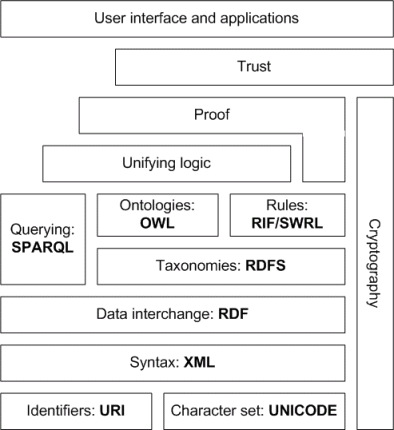
\includegraphics[scale=0.5]{Semantic-web-stack.png}
\caption{Semantic-web-stack}
\label{Semantic-web-stack}
\end{figure}

\subsection{Current state of standardization}

Well-established standards:

\begin{compactitem}
\item Unicode
\item Uniform Resource Identifier
\item XML
\item RDF
\item RDFS
\item SPARQL
\item Web Ontology Language (OWL)
\item Rule Interchange Format (RIF)
\end{compactitem}

Not yet fully realized:

\begin{compactitem}
\item Unifying Logic and Proof layers
\end{compactitem}

The intent is to enhance the usability and usefulness of the Web and its interconnected resources through:

\begin{compactitem}
\item Servers which expose existing data systems using the RDF and SPARQL standards. Many converters to RDF exist from different applications. Relational databases are an important source. The semantic web server attaches to the existing system without affecting its operation.
\item Documents "marked up" with semantic information (an extension of the HTML <meta> tags used in today's Web pages to supply information for Web search engines using web crawlers). This could be machine-understandable information about the human-understandable content of the document (such as the creator, title, description, etc.) or it could be purely metadata representing a set of facts (such as resources and services elsewhere on the site). Note that anything that can be identified with a Uniform Resource Identifier (URI) can be described, so the semantic web can reason about animals, people, places, ideas, etc. Semantic markup is often generated automatically, rather than manually.
\item Common metadata vocabularies (ontologies) and maps between vocabularies that allow document creators to know how to mark up their documents so that agents can use the information in the supplied metadata (so that Author in the sense of 'the Author of the page' won't be confused with Author in the sense of a book that is the subject of a book review)
\item Automated agents to perform tasks for users of the semantic web using this data
\item Web-based services (often with agents of their own) to supply information specifically to agents, for example, a Trust service that an agent could ask if some online store has a history of poor service or spamming
\end{compactitem}




\section{Skeptional reactions}


\subsection{Practical feasibility}

Critics (e.g. Which Semantic Web) question the basic feasibility of a complete or even partial fulfillment of the semantic web. Cory Doctorow's critique ("metacrap") is from the perspective of human behavior and personal preferences. For example, people may include spurious metadata into Web pages in an attempt to mislead Semantic Web engines that naively assume the metadata's veracity. This phenomenon was well-known with metatags that fooled the AltaVista ranking algorithm into elevating the ranking of certain Web pages: the Google indexing engine specifically looks for such attempts at manipulation. Peter Gärdenfors and Timo Honkela point out that logic-based semantic web technologies cover only a fraction of the relevant phenomena related to semantics.

Core, specialized communities and organizations for intra-company projects tended to practically adopt semantic web technologies greater than peripheral and less-specialized communities.[29] The practical constraints toward adoption have appeared less challenging where domain and scope is more limited than that of the general public and the World-Wide Web.[29]


\subsection{Censorship and privacy}

Enthusiasm about the semantic web could be tempered by concerns regarding censorship and privacy. For instance, text-analyzing techniques can now be easily bypassed by using other words, metaphors for instance, or by using images in place of words. An advanced implementation of the semantic web would make it much easier for governments to control the viewing and creation of online information, as this information would be much easier for an automated content-blocking machine to understand. In addition, the issue has also been raised that, with the use of FOAF files and geo location meta-data, there would be very little anonymity associated with the authorship of articles on things such as a personal blog. Some of these concerns were addressed in the "Policy Aware Web" project[30] and is an active research and development topic.

\subsection{Doubling output formats}

Another criticism of the semantic web is that it would be much more time-consuming to create and publish content because there would need to be two formats for one piece of data: one for human viewing and one for machines. However, many web applications in development are addressing this issue by creating a machine-readable format upon the publishing of data or the request of a machine for such data. The development of microformats has been one reaction to this kind of criticism. Another argument in defense of the feasibility of semantic web is the likely falling price of human intelligence tasks in digital labor markets, such as the Amazon Mechanical Turk.

Specifications such as eRDF and RDFa allow arbitrary RDF data to be embedded in HTML pages. The GRDDL (Gleaning Resource Descriptions from Dialects of Language) mechanism allows existing material (including microformats) to be automatically interpreted as RDF, so publishers only need to use a single format, such as HTML.


\section{Projects}

This section lists some of the many projects and tools that exist to create Semantic Web solutions.


\subsection{DBpedia}

DBPedia is an effort to publish structured data extracted from Wikipedia: the data is published in RDF and made available on the Web for use under the GNU Free Documentation License, thus allowing Semantic Web agents to provide inferencing and advanced querying over the Wikipedia-derived dataset and facilitating interlinking, re-use and extension in other data-sources.



\subsection{FOAF}

A popular vocabulary on the semantic web is Friend of a Friend (or FOAF), which uses RDF to describe the relationships people have to other people and the "things" around them. FOAF permits intelligent agents to make sense of the thousands of connections people have with each other, their jobs and the items important to their lives; connections that may or may not be enumerated in searches using traditional web search engines. Because the connections are so vast in number, human interpretation of the information may not be the best way of analyzing them.

FOAF is an example of how the Semantic Web attempts to make use of the relationships within a social context.

\subsection{SIOC}

The Semantically-Interlinked Online Communities project (SIOC, pronounced "shock") provides a vocabulary of terms and relationships that model web data spaces. Examples of such data spaces include, among others: discussion forums, blogs, blogrolls / feed subscriptions, mailing lists, shared bookmarks and image galleries.


\subsection{GoPubMed}

GoPubMed is a knowledge-based search engine for biomedical texts. The Gene Ontology (GO) and Medical Subject Headings (MeSH) serve as "Table of contents" in order to structure the millions of articles of the MEDLINE database. The search engine allows its users to find relevant search results significantly faster than Pubmed.


\subsection{NextBio}

A database consolidating high-throughput life sciences experimental data tagged and connected via biomedical ontologies. Nextbio is accessible via a search engine interface. Researchers can contribute their findings for incorporation to the database. The database currently supports gene expression or protein expression data and sequence centric data and is steadily expanding to support other biological data types.













\chapter{Delivery}

HTML documents can be delivered by the same means as any other computer file. However, they are most often delivered either by HTTP from a web server or by email.

\begin{compactitem}
\item HTTP

The World Wide Web is composed primarily of HTML documents transmitted from web servers to web browsers using the Hypertext Transfer Protocol (HTTP). However, HTTP is used to serve images, sound, and other content, in addition to HTML. To allow the web browser to know how to handle each document it receives, other information is transmitted along with the document. This meta data usually includes the MIME type (e.g. text/html or application/xhtml+xml) and the character encoding (see Character encoding in HTML).

In modern browsers, the MIME type that is sent with the HTML document may affect how the document is initially interpreted. A document sent with the XHTML MIME type is expected to be well-formed XML; syntax errors may cause the browser to fail to render it. The same document sent with the HTML MIME type might be displayed successfully, since some browsers are more lenient with HTML.

The W3C recommendations state that XHTML 1.0 documents that follow guidelines set forth in the recommendation's Appendix C may be labeled with either MIME Type. XHTML 1.1 also states that XHTML 1.1 documents should[59] be labeled with either MIME type.

万维网主要由从服务器通过HTTP协议向浏览器发送的HTML文档组成。但是,HTTP也可以被用于传输HTML之外的数据,例如图像、声音和其他内容。为使浏览器了解如何处理接收到的文档,在传输文档时必须同时传递文件类型。这种元数据包含MIME类型(对于HTML 4.01或更早版本是text/html,而对于XHTML 1.0或之后的版本是application/xhtml+xml),以及字符编码。

在现在的浏览器中,和HTML文档一起发送的MIME类型影响文档的解读方式。和XHTML MIME类型一起发送的文档被认为是良构的XML,而语法错误会导致浏览器无法呈现文档。完全相同的文档如果和HTML MIME类型一起发送,则可能被正常显示,因为浏览器对HTML的语法检查更加松懈些。

\item HTML e-mail

Most graphical email clients allow the use of a subset of HTML (often ill-defined) to provide formatting and semantic markup not available with plain text. This may include typographic information like coloured headings, emphasized and quoted text, inline images and diagrams. Many such clients include both a GUI editor for composing HTML e-mail messages and a rendering engine for displaying them. Use of HTML in e-mail is controversial because of compatibility issues, because it can help disguise phishing attacks, because of accessibility issues for blind or visually impaired people, because it can confuse spam filters and because the message size is larger than plain text.

一些图形模式下的电子邮件客户端支持HTML格式的邮件。很多支持一个图形模式下的HTML邮件编辑器,以及一个HTML邮件阅览器。因为一些问题,HTML邮件的使用有争议。HTML邮件的主要优点是可以使用呈现性元素来加强邮件的视觉效果,但是缺陷也很多,例如:

\begin{compactitem}
\item 收件人未必有一个可以浏览HTML邮件的客户端
\item 邮件大小增加。一些邮件客户端随HTML邮件发送一个纯文字版更加重了这个问题
\item 过度使用格式化
\item 潜在安全问题,例如伪造银行电子邮件用于网络钓鱼
\item 在一些有缺陷的电子邮件程序显示HTML邮件时可能执行恶意代码
\end{compactitem}

因为这些原因,很多新闻组和邮件列表要么截断信件的HTML部分,要么只接受纯文本版本部分的邮件,要么拒绝接收HTML邮件。

\item Naming conventions

The most common filename extension for files containing HTML is .html. A common abbreviation of this is .htm, which originated because some early operating systems and file systems, such as DOS and the limitations imposed by FAT data structure, limited file extensions to three letters.

\item HTML Application

An HTML Application (HTA; file extension ".hta") is a Microsoft Windows application that uses HTML and Dynamic HTML in a browser to provide the application's graphical interface. A regular HTML file is confined to the security model of the web browser's security, communicating only to web servers and manipulating only webpage objects and site cookies. An HTA runs as a fully trusted application and therefore has more privileges, like creation/editing/removal of files and Windows Registry entries. Because they operate outside the browser's security model, HTAs cannot be executed via HTTP, but must be downloaded (just like an EXE file) and executed from local file system .

\end{compactitem}





\chapter{Current variations}

Since its inception, HTML and its associated protocols gained acceptance relatively quickly. However, no clear standards existed in the early years of the language. Though its creators originally conceived of HTML as a semantic language devoid of presentation details, practical uses pushed many presentational elements and attributes into the language, driven largely by the various browser vendors. The latest standards surrounding HTML reflect efforts to overcome the sometimes chaotic development of the language[64] and to create a rational foundation for building both meaningful and well-presented documents. To return HTML to its role as a semantic language, the W3C has developed style languages such as CSS and XSL to shoulder the burden of presentation. In conjunction, the HTML specification has slowly reined in the presentational elements.


There are two axes differentiating various variations of HTML as currently specified: SGML-based HTML versus XML-based HTML (referred to as XHTML) on one axis, and strict versus transitional (loose) versus frameset on the other axis.


\section{SGML-based versus XML-based HTML}


One difference in the latest HTML specifications lies in the distinction between the SGML-based specification and the XML-based specification. The XML-based specification is usually called XHTML to distinguish it clearly from the more traditional definition. However, the root element name continues to be 'html' even in the XHTML-specified HTML. The W3C intended XHTML 1.0 to be identical to HTML 4.01 except where limitations of XML over the more complex SGML require workarounds. Because XHTML and HTML are closely related, they are sometimes documented in parallel. In such circumstances, some authors conflate the two names as (X)HTML or X(HTML).

Like HTML 4.01, XHTML 1.0 has three sub-specifications: strict, transitional and frameset.

Aside from the different opening declarations for a document, the differences between an HTML 4.01 and XHTML 1.0 document—in each of the corresponding DTDs—are largely syntactic. The underlying syntax of HTML allows many shortcuts that XHTML does not, such as elements with optional opening or closing tags, and even EMPTY elements which must not have an end tag. By contrast, XHTML requires all elements to have an opening tag and a closing tag. XHTML, however, also introduces a new shortcut: an XHTML tag may be opened and closed within the same tag, by including a slash before the end of the tag like this: <br/>. The introduction of this shorthand, which is not used in the SGML declaration for HTML 4.01, may confuse earlier software unfamiliar with this new convention. A fix for this is to include a space before closing the tag, as such: <br />.

To understand the subtle differences between HTML and XHTML, consider the transformation of a valid and well-formed XHTML 1.0 document that adheres to Appendix C (see below) into a valid HTML 4.01 document. To make this translation requires the following steps:

\begin{compactenum}
\item The language for an element should be specified with a lang attribute rather than the XHTML xml:lang attribute. XHTML uses XML's built in language-defining functionality attribute.
\item Remove the XML namespace (xmlns=URI). HTML has no facilities for namespaces.
\item Change the document type declaration from XHTML 1.0 to HTML 4.01. (see DTD section for further explanation).
\item If present, remove the XML declaration. (Typically this is: <?xml version="1.0" encoding="utf-8"?>).
\item Ensure that the document's MIME type is set to text/html. For both HTML and XHTML, this comes from the HTTP Content-Type header sent by the server.
\item Change the XML empty-element syntax to an HTML style empty element (<br/> to <br>).

\end{compactenum}
Those are the main changes necessary to translate a document from XHTML 1.0 to HTML 4.01. To translate from HTML to XHTML would also require the addition of any omitted opening or closing tags. Whether coding in HTML or XHTML it may just be best to always include the optional tags within an HTML document rather than remembering which tags can be omitted.

A well-formed XHTML document adheres to all the syntax requirements of XML. A valid document adheres to the content specification for XHTML, which describes the document structure.

The W3C recommends several conventions to ensure an easy migration between HTML and XHTML (see HTML Compatibility Guidelines). The following steps can be applied to XHTML 1.0 documents only:

\begin{compactitem}
\item Include both xml:lang and lang attributes on any elements assigning language.
\item Use the empty-element syntax only for elements specified as empty in HTML.
\item Include an extra space in empty-element tags: for example <br /> instead of <br/>.
\item Include explicit close tags for elements that permit content but are left empty (for example, <div></div>, not <div />).
\item Omit the XML declaration.
\end{compactitem}

By carefully following the W3C's compatibility guidelines, a user agent should be able to interpret the document equally as HTML or XHTML. For documents that are XHTML 1.0 and have been made compatible in this way, the W3C permits them to be served either as HTML (with a text/html MIME type), or as XHTML (with an application/xhtml+xml or application/xml MIME type). When delivered as XHTML, browsers should use an XML parser, which adheres strictly to the XML specifications for parsing the document's contents.



\section{Transitional versus strict}

HTML 4 defined three different versions of the language: Strict, Transitional (once called Loose) and Frameset. The Strict version is intended for new documents and is considered best practice, while the Transitional and Frameset versions were developed to make it easier to transition documents that conformed to older HTML specification or didn't conform to any specification to a version of HTML 4. The Transitional and Frameset versions allow for presentational markup, which is omitted in the Strict version. Instead, cascading style sheets are encouraged to improve the presentation of HTML documents. Because XHTML 1 only defines an XML syntax for the language defined by HTML 4, the same differences apply to XHTML 1 as well.

The Transitional version allows the following parts of the vocabulary, which are not included in the Strict version:

\begin{compactitem}

\item A looser content model

	\begin{compactitem}
	\item Inline elements and plain text are allowed directly in: body, blockquote, form, noscript and noframes
	\end{compactitem}

\item Presentation related elements
	
	\begin{compactitem}
	\item underline (u)(Deprecated. can confuse a visitor with a hyperlink.)
	\item strike-through (s)
	\item center (Deprecated. use CSS instead.)
	\item font (Deprecated. use CSS instead.)
	\item basefont (Deprecated. use CSS instead.)
	\end{compactitem}
	
\item Presentation related attributes
	\begin{compactitem}
	\item background (Deprecated. use CSS instead.) and bgcolor (Deprecated. use CSS instead.)  attributes for body (required element according to the W3C.) element.
	\item align (Deprecated. use CSS instead.) attribute on div, form, paragraph (p) and heading (h1...h6) elements
	\item align (Deprecated. use CSS instead.), noshade (Deprecated. use CSS instead.), size (Deprecated. use CSS instead.) and width (Deprecated. use CSS instead.) attributes on hr element
	\item align (Deprecated. use CSS instead.), border, vspace and hspace attributes on img and object (caution: the object element is only supported in Internet Explorer (from the major browsers)) elements
	\item align (Deprecated. use CSS instead.) attribute on legend and caption elements
	\item align (Deprecated. use CSS instead.) and bgcolor (Deprecated. use CSS instead.) on table element
	\item nowrap (Obsolete), bgcolor (Deprecated. use CSS instead.), width, height on td and th elements
	\item bgcolor (Deprecated. use CSS instead.) attribute on tr element
	\item clear (Obsolete) attribute on br element
	\item compact attribute on dl, dir and menu elements
	\item type (Deprecated. use CSS instead.), compact (Deprecated. use CSS instead.) and start (Deprecated. use CSS instead.) attributes on ol and ul elements
	\item type and value attributes on li element
	\item width attribute on pre element
	\end{compactitem}
	
\item Additional elements in Transitional specification
	
	\begin{compactitem}
	\item menu (Deprecated. use CSS instead.) list (no substitute, though unordered list is recommended)
	\item dir (Deprecated. use CSS instead.) list (no substitute, though unordered list is recommended)
	\item isindex (Deprecated.) (element requires server-side support and is typically added to documents server-side, form and input elements can be used as a substitute)
	\item applet (Deprecated. use the object element instead.)
	\end{compactitem}

\item The language (Obsolete) attribute on script element (redundant with the type attribute).
\item Frame related entities
	\begin{compactitem}
	\item iframe
	\item noframes
	\item target (Deprecated in the map, link and form elements.) attribute on a, client-side image-map (map), link, form and base elements
	\end{compactitem}
	
\end{compactitem}

The Frameset version includes everything in the Transitional version, as well as the frameset element (used instead of body) and the frame element.



\section{Frameset versus transitional}

In addition to the above transitional differences, the frameset specifications (whether XHTML 1.0 or HTML 4.01) specifies a different content model, with frameset replacing body, that contains either frame elements, or optionally noframes with a body.



\section{Summary of specification versions}

As this list demonstrates, the loose versions of the specification are maintained for legacy support. However, contrary to popular misconceptions, the move to XHTML does not imply a removal of this legacy support. Rather the X in XML stands for extensible and the W3C is modularizing the entire specification and opening it up to independent extensions. The primary achievement in the move from XHTML 1.0 to XHTML 1.1 is the modularization of the entire specification. The strict version of HTML is deployed in XHTML 1.1 through a set of modular extensions to the base XHTML 1.1 specification. Likewise, someone looking for the loose (transitional) or frameset specifications will find similar extended XHTML 1.1 support (much of it is contained in the legacy or frame modules). The modularization also allows for separate features to develop on their own timetable. So for example, XHTML 1.1 will allow quicker migration to emerging XML standards such as MathML (a presentational and semantic math language based on XML) and XForms—a new highly advanced web-form technology to replace the existing HTML forms.

In summary, the HTML 4 specification primarily reined in all the various HTML implementations into a single clearly written specification based on SGML. XHTML 1.0, ported this specification, as is, to the new XML defined specification. Next, XHTML 1.1 takes advantage of the extensible nature of XML and modularizes the whole specification. XHTML 2.0 was intended to be the first step in adding new features to the specification in a standards-body-based approach.


\section{WhatWG HTML versus HTML5}


The WhatWG considers their work as living standard HTML for what constitutes the state of the art in major browser implementations by Apple (Safari), Google (Chrome), Mozilla (Firefox), Opera (Opera), and others. HTML5 is specified by the HTML Working Group of the W3C following the W3C process. As of 2013 both specifications are similar and mostly derived from each other, i.e., the work on HTML5 started with an older WhatWG draft, and later the WhatWG living standard was based on HTML5 drafts in 2011.









\chapter{Hypertext features not in HTML}

HTML lacks some of the features found in earlier hypertext systems, such as source tracking, fat links and others. Even some hypertext features that were in early versions of HTML have been ignored by most popular web browsers until recently, such as the link element and in-browser Web page editing.

Sometimes Web services or browser manufacturers remedy these shortcomings. For instance, wikis and content management systems allow surfers to edit the Web pages they visit.

HTML是一个相对比较弱的超文本实现。早期超文本系统具有具有类型的链接、跨越包含和来源跟踪这样的属性。另一个现在缺乏支持的特性是粗链路。

直到不久之前,一些早期HTML版本中的超文本特性一直被大多数浏览器忽略,例如link元素和可编辑的网页。

有时网络服务或者浏览器厂商也认识到这些特性。例如,现在的wiki和nuke社会网络软件允许浏览者编辑访问的网页。

\chapter{HTML editor}

An HTML editor is a computer program for creating web pages. Although the HTML markup of a web page can be written with any text editor, specialized HTML editors can offer convenience and added functionality. For example, many HTML editors work not only with HTML, but also with related technologies such as CSS, XML and JavaScript or ECMAScript. In some cases they also manage communication with remote web servers via FTP and WebDAV, and version management systems such as CVS or Subversion.

There are various forms of HTML editors: text, object and WYSIWYG (what you see is what you get) editors.


\section{Text editors}

Text (source) editors intended for use with HTML usually provide syntax highlighting. Templates, toolbars and keyboard shortcuts may quickly insert common HTML elements and structures. Wizards, tooltip prompts and autocompletion may help with common tasks.

Text HTML editors commonly include either built-in functions or integration with external tools for such tasks as source and version control, link-checking, code checking and validation, code cleanup and formatting, spell-checking, uploading by FTP or WebDAV, and structuring as a project.

Text editors require user understanding of HTML and any other web technologies the designer wishes to use like CSS, JavaScript and server-side scripting languages. They were also referred to A Simple HTML Editor (ASHE).

Some regular text editors such as Windows Notepad can save as HTML files simply by using extensions such as .html .htm .css etc.


\section{Object editors}

Some editors allow alternate editing of the source text of objects in more visually organized modes than simple color highlighting, but in modes not considered WYSIWYG. Some WYSIWYG editors include the option of using palette windows that enable editing the text-based parameters of selected objects. These palettes allow either editing parameters in fields for each individual parameter, or text windows to edit the full group of source text for the selected object. They may include widgets to present and select options when editing parameters. Adobe GoLive provides an outline editor to expand and collapse HTML objects and properties, edit parameters, and view graphics attached to the expanded objects.




\section{WYSIWYG editors}

There are some WYSIWYG (What You See Is What You Get) editors, in which the user lays out everything as it is to appear in the HTML document using a graphical user interface (GUI), often similar to word processors. The editor renders the document rather than show the code, so authors do not require extensive knowledge of HTML.



The WYSIWYG editing model has been criticized, primarily because of the low quality of the generated code; there are voices advocating a change to the WYSIWYM model (What You See Is What You Mean).

WYSIWYG HTML editors provide an editing interface which resembles how the page will be displayed in a web browser. These editors may be stand-alone programs, such as Adobe Dreamweaver or Microsoft Frontpage, or come in the form of browser extensions and allow editing directly within the web browser. Because using a WYSIWYG editor may not require any HTML knowledge, they are often easier for an average computer user to get started with.

WYSIWYG editors remain a controversial topic because of their perceived flaws such as:

\begin{compactitem}
\item Relying mainly on layout as opposed to meaning, often using markup that does not convey the intended meaning but simply copies the layout.
\item Often producing extremely verbose and redundant code that fails to make use of the cascading nature of HTML and CSS.
\item Often producing ungrammatical markup often called tag soup or semantically incorrect markup (such as <em> for italics).
\item As a great deal of the information in HTML documents is not in the layout, the model has been criticized for its "what you see is all you get"-nature
\end{compactitem}

The WYSIWYG view is achieved by embedding a layout engine based upon that used in a web browser. The layout engine will have been considerably enhanced by the editor's developers to allow for typing, pasting, deleting and manipulation of the content. The goal is that, at all times during editing, the rendered result should represent what will be seen later in a typical web browser.

\section{WYSIWYM editors}

WYSIWYM (what you see is what you mean) is an alternative paradigm to the WYSIWYG editors above. Instead of focusing on the format or presentation of the document, it preserves the intended meaning of each element. For example, page headers, sections, paragraphs, etc. are labeled as such in the editing program, and displayed appropriately in the browser.

\section{Online editors}

There are many online WYSIWYG HTML editors, some of them are:

\begin{compactitem}
\item CLEditor
\item CKEditor
\item OpenBEXI
\item SnapEditor
\item TinyMCE
\item WYMeditor
\item YUI Rich Text Editor
\end{compactitem}

\section{Difficulties in achieving WYSIWYG}


A given HTML document will have an inconsistent appearance on various platforms and computers for several reasons:

\begin{compactitem}
\item Different browsers and applications will render the same markup differently.

The same page may display slightly differently in Internet Explorer and Firefox on a high-resolution screen, but it will look very different in the perfectly valid text-only Lynx browser. It needs to be rendered differently again on a PDA, an internet-enabled television and on a mobile phone. Usability in a speech or braille browser, or via a screen-reader working with a conventional browser, will place demands on entirely different aspects of the underlying HTML. Printing the page, via different browsers and different printers onto various paper sizes, around the world, places other demands. With the correct use of modern HTML and CSS there is no longer any need to provide 'Printable page' links and then have to maintain two versions of the whole site. Nor is there any excuse for pages not fitting the user's preferred paper size and orientation, or wasting ink printing solid background colours unnecessarily, or wasting paper reproducing navigation panels that will be entirely useless once printed out.

\item Browsers and computer graphics systems have a range of user settings.

Resolution, font size, colour, contrast etc can all be adjusted at the user's discretion, and many modern browsers allow even more user control over page appearance. All an author can do is suggest an appearance.

\item Web browsers, like all computer software, have bugs

They may not conform to current standards. It is hopeless to try to design Web pages around all of the common browsers' current bugs: each time a new version of each browser comes out, a significant proportion of the World Wide Web would need re-coding to suit the new bugs and the new fixes. It is generally considered much wiser to design to standards, staying away from 'bleeding edge' features until they settle down, and then wait for the browser developers to catch up to your pages, rather than the other way round. For instance, no one can argue that CSS is still 'cutting edge' as there is now widespread support available in common browsers for all the major features, even if many WYSIWYG and other editors have not yet entirely caught up.

\item A single visual style can represent multiple semantic meanings

Semantic meaning, derived from the underlying structure of the HTML document, is important for search engines and also for various accessibility tools. On paper we can tell from context and experience whether bold text represents a title, or emphasis, or something else. But it is very difficult to convey this distinction in a WYSIWYG editor. Simply making a piece of text bold in a WYSIWYG editor is not sufficient to tell the editor *why* the text is bold - what the boldness represents semantically.

\end{compactitem}

What you see may be what most visitors get, but it is not guaranteed to be what everyone gets.



\chapter{HTML Parser}

Parsing HTML is a automated task, performed by (so called) HTML parsers. They have two main purposes:

\begin{compactitem}
\item HTML traversal

offer a interface for programmers to easily access and modify of the "HTML string code". Canonical example: DOM parsers.
\item HTML clean

To fix invalid HTML and to improve the layout and indent style of the resulting markup. Canonical example: HTML Tidy.
\end{compactitem}







































